The model developed by White~\cite{white87} and later refined for \gls{har} by Fu et al.~\cite{sensing-survey} 
can be used to categorize sensors and data modalities recorded by them.
To produce a versatile data set, 
multiple data modalities should be included.
This requires the inclusion of multiple devices in the array.
The categorization model is presented in Figure \ref{fig:sensor-categories}.

The sensors used for the system, with the recorded modalities and highlight colour in parentheses,
were the following:
\begin{itemize}
    \item Texas Instruments IWR6843ISK + DCA1000EVM (radar, cyan),
    \item Panasonic Grid-EYE (infrared, yellow),
    \item Intel RealSense D435i (RGB-D video, red), and
    \item MiniDSP UMA-16 (acoustic, green).
\end{itemize}

The modalities recorded by the sensors are highlighted in different colours in Figure \ref{fig:sensor-categories}.
From the figure, it can be observed that three out of five sensor categories are present,
and from the present sensor categories all but three modalities can be recorded.
Most of the excluded sensors are rather laborious to install in contrast to the included sensors.
Capacitive sensing only works on ranges up to half a meter,
ambient temperature sensing provides very minimal information about human activities,
and magnetic sensing requires a large number of sensors compared to the useful information gained from them.
The excluded acoustic sensors could provide useful information with very little installation cost.
WiFi based electromagnetic sensing could also potentially bring more value to the system,
but radar can detect movements with a much finer resolution and the radar devices are perhaps easier to interface with.~\cite{sensing-survey}
All in all, most of the interesting data modalities are recorded by the sensors in the system,
with some room for improvement.

\begin{figure}[H]
    \centering
    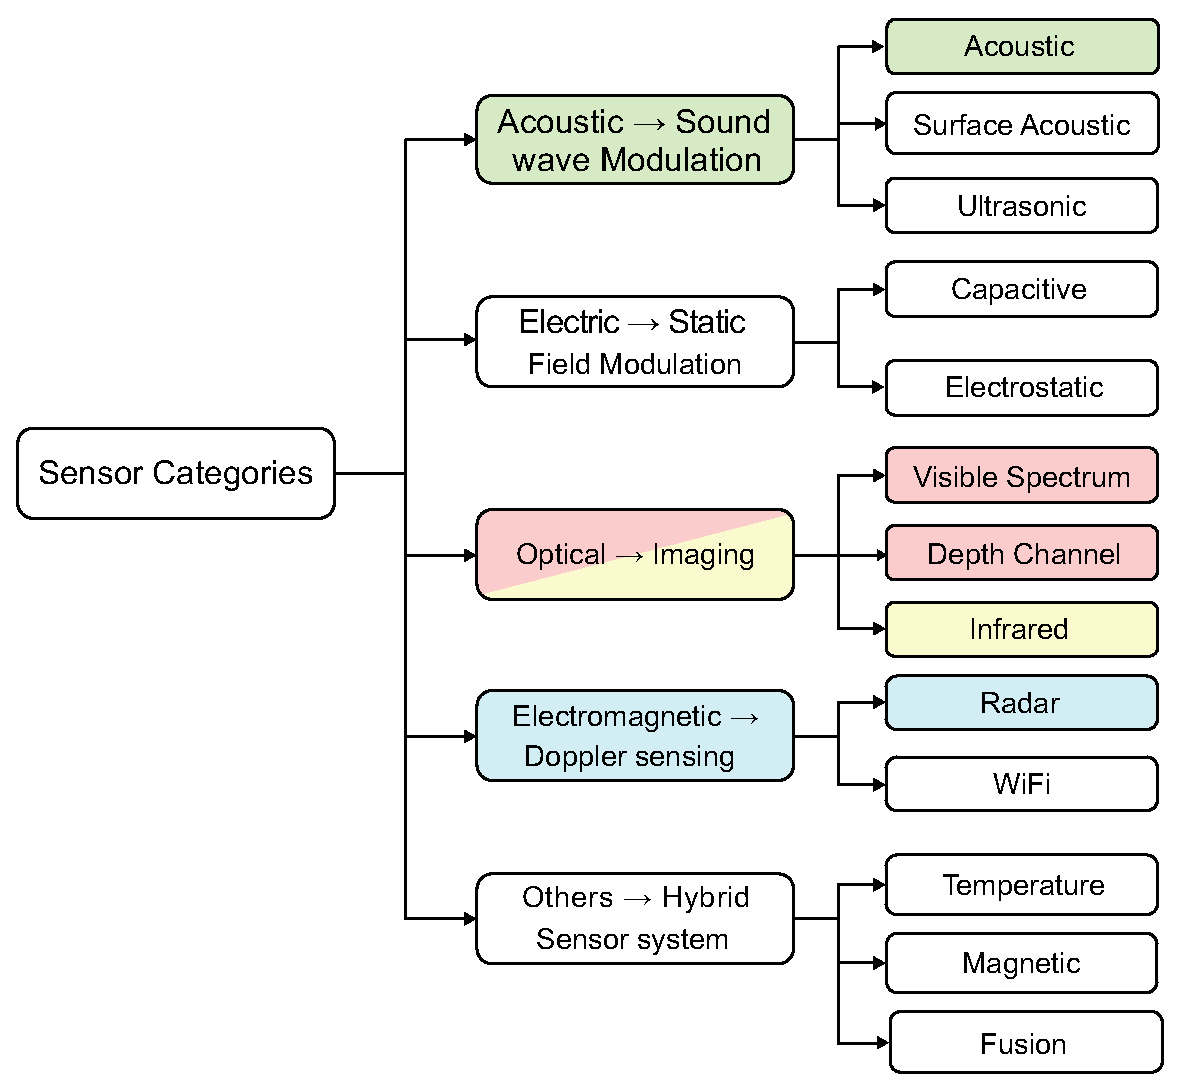
\includegraphics[width=0.7\textwidth]{fig/2/sensor-categories.eps}
    \caption{
        Sensor categorization model by Fu et al.~\cite{sensing-survey}.
        Data modalities present in the data collection system of this thesis are highlighted in different colours.
    }
    \label{fig:sensor-categories}
\end{figure}

The sensors are mounted on a single steel plate,
giving them an uniform perspective to the target.
The mounting bracket can be attached to a standard camera tri-pod.
The system is very portable as the sensors can be connected via USB to a computer,
and only two of the devices require an external power source:
USB cannot deliver enough power for the radar device, and the microphone requires a 12-volt input voltage.

The mounting bracket and the positions of the sensors on it are illustrated in Figure \ref{fig:sensor-array}.
The mounting bracket is drawn in white.
The blue outline represents the components of the radar device,
yellow outline represents the infrared camera,
red outline represents the RGB-D camera,
and the green outline represents the microphone.
The deeper-coloured circles represent the screw holes the sensors were mounted on.
The white circle represents the tri-pod attachment point.

\begin{figure}[H]
    \centering
    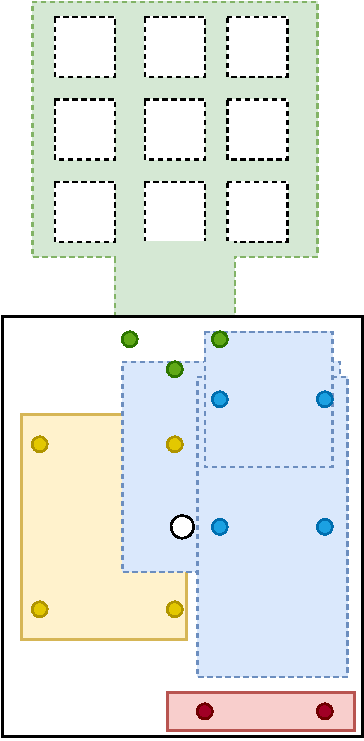
\includegraphics{fig/3/sensor-array.pdf}
    \caption{The sensor array illustrated, not in scale.}
    \label{fig:sensor-array}
\end{figure}

With the sensors chosen,
before a data collection campaign can ensue,
software needs to be written to interface with the sensors and to record the data produced by them.
The contribution of this thesis in the data collection project is to develop this software.

The following sections (\ref{sec:2-radar}--\ref{sec:2-mic}) will discuss the operating characteristics, connection interfaces,
and recorded data modalities of the included sensors.
Finally, Section \ref{sec:2-requirements} will discuss the requirements
and evaluation criteria for the data collection software developed for this thesis.

\section{Radar}
\label{sec:2-radar}
The radar used in the assembly is a Texas Instruments IWR6843ISK mmWave radar evaluation board.
It is capable of outputting various continuous radar signals.
It operates on 60--64 GHz frequency and has a maximum of 120-degree horizontal \gls{fov} and 30-degree vertical \gls{fov}.
It has a monostatic radar with distinct transmitting and receiving antennas mounted side-by-side.
The receiving antenna is a uniform linear array that consists of four antennas with 1/2-wavelength separation.
The transmitting antenna consists of three antennas, also separated by 1/2-wavelength.
The transmitting antenna is non-linear with the middle antenna slightly raised.
The antennas are illustrated in figure \ref{fig:antennas}.

\begin{figure}[H]
    \centering
    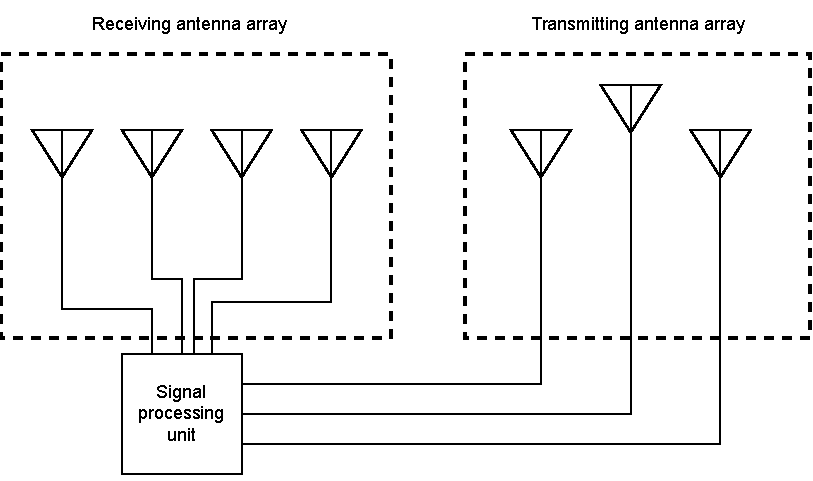
\includegraphics[width=0.8\textwidth]{fig/3/antennas.pdf}
    \caption{Antenna arrays illustrated. More detailed documentation is available in the device user guide~\cite{ti-iwr-user-guide}.}
    \label{fig:antennas}
\end{figure}

When multiple active receivers are used,
the location of the target can be detected in all three dimensions by applying angle and distance estimation algorithms,
such as the \gls{2d-music} and \gls{2d-fft} algorithms (Sections \ref{sec:range-angle}--\ref{sec:cfar}).
The receivers can be toggled on and off from a special configuration file.
The same configuration file can be used to define nearly arbitrary signal formats~\cite{mmwave-sdk-user-guide}.

The IRW6843ISK is capable of processing the radar samples into radar frames on-board,
but but depending on the operating parameters,
its performance is limited to around 1--4 frames per second.
To get more performance out of the device,
the DCA1000EVM is used to interface with the IWR6843ISK to record the raw samples without processing them on-board.
The processing is instead done separately by external software to form the radar frames.

\begin{figure}[H]
    \centering
    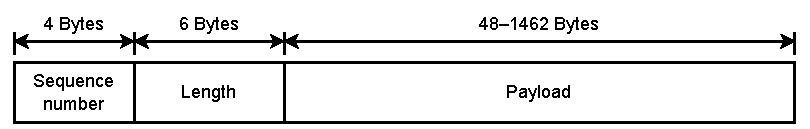
\includegraphics[width=0.9\textwidth]{fig/2/radar-frame-bytes.pdf}
    \caption{The structure of the data frames output by the DCA1000EVM.}
    \label{fig:radar-frame-bytes}
\end{figure}

The DCA1000EVM outputs the radar samples in a rather complicated format,
that is documented in detail in the user guide for the device.
The frames output by the device depend on its configured operating mode.
In this system, the device is configured in such a way that the frames consist of a 4-byte sequence number,
6-byte length field and a 48--1462-byte payload (Figure \ref{fig:radar-frame-bytes})~\cite{dca1000-user-guide}.

\begin{figure}[H]
    \centering
    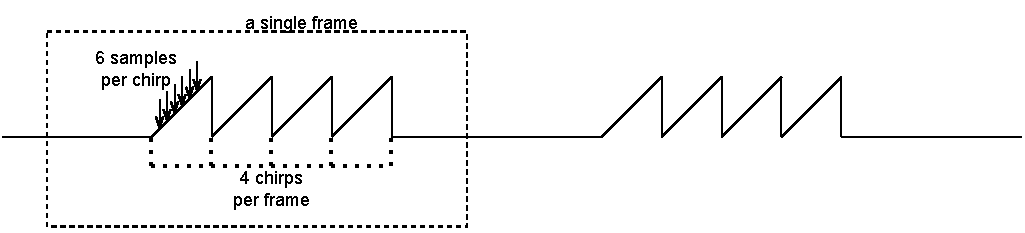
\includegraphics[width=0.9\textwidth]{fig/2/2-radar-sampling.pdf}
    \caption{Illustration of samples, chirps, and frames. With 2 receiving antennas,
    the equation \ref{eq:bytes-per-frame} would give $N_{\mathrm{total}} = 4\cdot6\cdot4\cdot2 = 192$ bytes per frame.
    In a practical situation, the numbers would, of course, be much higher.}
    \label{fig:2-radar-signal-sampling}
\end{figure}

The data field of the frames consist of 2-byte complex samples,
that can be arranged to 4-byte I/Q samples~\cite{dca1000-raw-data-capture},
i.e. four bytes of data are output for each sample.
The number of samples in a single radar frame \gls{total-samples} can be calculated as given by equation \ref{eq:bytes-per-frame},
\gls{numsamples} is the number of samples per chirp,
\gls{numchirps} is the number of chirps per frame,
and \gls{numrcv} is the number of active receiving antennas.
Figure \ref{fig:2-radar-signal-sampling} illustrates the formula.
The number of bytes per radar frame is $4 \gls{total-samples}$.

\begin{equation}
\label{eq:bytes-per-frame}
    \gls{total-samples} = 4 \gls{numsamples} \gls{numchirps}  \gls{numrcv},
\end{equation}


As the frames output by the DCA1000EVM do not correspond exactly to the \gls{total-samples}-byte radar frames,
the data segments should simply be concatenated in the order indicated by the sequence number until a full frame can be stored or processed.
The developed data collection software saves the data segments on disk as-is,
and the exact format of the data segments is presented in more detail in Section \ref{sec:radar-file}.

The radar sensor has proven to be effective in \gls{har}.
Unlike optical and acoustic sensors,
radar is insensitive to environmental factors such as weather, lightning and acoustic noise.
It is also capable of sensing through most (non-conductive) walls,
making it less prone to occlusion.
Using \gls{mmWave} frequencies, radar is capable of detecting movements even in the sub-millimeter range.

After processing, various information can can be extracted from the data:
\begin{itemize}
    \item target range, azimuth and altitude angle (Section \ref{sec:range-angle}),
    \item range-velocity spectrum (Section \ref{sec:doppler-spectrum}), and
    \item radar cross-section.
\end{itemize}
From \gls{har} perspective, the first three items of the list are the most interesting,
especially the doppler-spectrum (time-frequency spectrogram)~\cite{sensing-survey}.

The radar can effectively detect various activities based on the Doppler-spectrum~\cite{bumblebee-micro-doppler-har, seifert19, liu12, kim16}.
Additionally it can very effectively measure the location of a target,
which can be used as additional information for other sensors.
As a downside, radar devices are very expensive and power-consuming.
This can limit its usefulness in low-power or low-budget applications.

\section{Optical}
The optical sensors consist of conventional visible spectrum imaging (RGB video),
depth imaging, and infrared imaging.
The system in this thesis includes sensors that can record all these modalities.
The Intel RealSense D435i is capable of both visual spectrum and depth imaging,
while the Panasonic Grid-EYE records the \gls{ir} spectrum.

Visible spectrum video is one of the best studied areas in computer vision and \gls{har}.
The primary approach to \gls{har} from RGB video is using convolutional neural networks.
Models such as AlexNet~\cite{alexnet}, and C3D have proven to be effective,
the latter reaching as high as 90 \% accuracy in detecting human actions~\cite{c3d}. 

Using a stereo camera, depth information can be extracted.
This allows for much simpler segmentation and pose estimation
compared to RGB video.~\cite{sensing-survey}
Combining the RGB and depth channels,
detection accuracies as high as 98 \% have been recorded on some data sets~\cite{cippitelli16}.

RGB video based segmentation and \gls{har} in general can be problematic in some scenarios.
If the image has poor contrast, proper segmentation may not be possible.
In addition to unfortunate colors,
this may be caused by bad lightning conditions, i.e. under- or overexposure or extreme fog.
Visible spectrum imaging also raises some privacy concerns in certain environments.

Thermal cameras are capable of detecting the heat radiation emitted from warm objects.
This makes them capable of detecting human motion from the background regardless of the lightning conditions~\cite{han05}.
Additionally, very low resolution (from 8x8 px to 16x16 px) \gls{ir} sensors
have been demonstrated to be capable of detecting human actions~\cite{10.1145/2632048.2636084}.
With a frame rate of 10 fps, detection accuracy of 85 \% and above has been reached depending on the action~\cite{sensing-survey, tao18}.
Although the detection accuracy is not as good as with the RGB-D camera,
the possibility of operating in any lightning conditions and with high respect to privacy
make the \gls{ir} camera a viable choice.

\subsection{RGB and Depth video}
The RGB and Depth modalities are provided by an Intel RealSense D435i RGB-D camera.
The D435i model uses a stereo camera aided by an infrared dot matrix to measure depth,
making it similar in operating principle to the popular Microsoft Kinect.

The depth camera has a 87-degree horizontal \gls{fov} and a 58-degree vertical \gls{fov}.
It can record up to 90 frames per second with up to 1280x720 pixel resolution.
The ideal operating range is 0.3--3.0 meters and the depth measurement error is <2\% at 2 meters.
The RGB camera has a 69-degree horizontal \gls{fov} and a 42-degree vertical \gls{fov}.
It can record at up to 1920x1080 resolution and up to 30 frames per second.~\cite{realsense-datasheet}

Intel provides a library that can be used to interface with the camera programmatically.
The library can be used natively from C++,
and wrappers are provided for multiple languages and toolkits,
perhaps most importantly Python, Matlab, and ROS (1 and 2).~\cite{librealsense2}
The Python wrapper was used in the data collection software.
It provides methods for getting the RGB-values, depth-values and time stamps of each frame~\cite{librealsense2-python-docs}.
 
\subsection{Infrared}
The \gls{ir} camera used in the assembly is the Panasonic GRID-EYE (part no. AMG8834).
It is an infrared camera with a resolution of 8-by-8 pixels.
It has both vertical and horizontal \gls{fov} of 60 degrees,
making each pixel 6-by-6 degrees.
It can operate in temperatures of 0--\SI{80}{\celsius},
and measure temperature with a resolution of \SI{0.5}{\celsius},
while the absolute temperature accuracy is 2.5--\SI{3.0}{\celsius}.
According to the manufacturer,
it can produce data at the rate of either 1 or 10 frames per second.~\cite{grid-eye-manual}
While developing the data collection software,
it was measured that the actual frame rate was approximately 8.62 frames per second, though.

The evaluation kit outputs data in 135-byte segments,
where the first 3 bytes are header bytes, followed by 130 bytes of data, and 2 bytes of tail (padding).
The first two bytes of the data represent the temperature 
of the internal thermistor of the device (ambient temperature)
and the following 128 bytes represent the \gls{ir} camera matrix packed in row-major order.
Temperatures are represented as multiples of four with little-endian two-byte integers.~\cite{grid-eye-protocol}
The real temperature is therefore the unpacked number divided by four.

\section{Audio}
\label{sec:2-mic}
The microphone used in the assembly is a MiniDSP UMA-16,
which is a 4-by-4 uniform rectangular array of microphones.
It is capable of sampling at up to 48 kHz.
Other possible sampling rates are 8, 11.025, 12, 16, 32, and 44.1 kHz.
The microphone uses 24-bit quantization.

The microphone connects to the computer via USB,
and can be interfaced with like any other microphone.
Multiple convenience libraries exist for interfacing with microphones via code.
Examples include SoundDevice (Python)~\cite{sounddevice-docs},
Simple DirectMedia Layer 2.0 (C, C\texttt{++}, C\#, Python)~\cite{SDL2}, and PortAudio (C, C\texttt{++})~\cite{portaudio}.

\section{Data recording software requirements}
\label{sec:2-requirements}

To produce a high-quality data set,
some requirements are also set for the software that ties the sensors together.
In addition to giving guidelines for developing the data collection software,
having defined requirements also allows evaluating the quality of the product.

As stated earlier in this chapter,
the sensor array could be improved by including some different sensors.
Therefore, the software must be extensible.
The latency between data generation and application of time stamps must also be minimized,
which calls for parallelism.
In addition to software design choices, there are some requirements for the data it produces.
The data shall:
\begin{itemize}
    \item be time-synchronized,
    \item be labelled,
    \item be well-structured, and
    \item include sufficient metadata.
\end{itemize}

Time synchronization, in the case of the data set,
means that the beginning of the data in each recorded modality
corresponds to the same point in time.
In other words, given a common starting time \gls{start-time},
the first data point should correspond to \gls{start-time} in each recorded modality.
In addition, the recorded data for any modality shall not end before a common ending time \gls{end-time}.
Given a known frame rate \gls{framerate},
satisfying this requirement allows easily mapping any moment in time (\gls{time}) to a frame number (\gls{framenumber}) (equation \ref{eq:time-to-sample}).

\begin{equation}
    \label{eq:time-to-sample}
    \gls{framenumber} = \lfloor \gls{framerate} \gls{time} \rfloor
\end{equation}

For the data to be useful in supervised learning,
the current activity at any given time must be included in the data set;
the data must be labelled.
Labelling can be done in various ways.

The most accurate labelling method is manual labelling:
someone goes over the data and applies appropriate labels to each activity.
Although this results in superior accuracy,
it is very laborious and therefore not very desirable.

The activities could also be sourced from some sensors and algorithms that are 
already capable of recognising activities with a high accuracy.
As previously stated, there are numerous algorithms that can recognize activities from RGB-D video.
The RGB-D video provided by the sensor array could therefore be used to map labels for the activities on the time domain.
Using equation \ref{eq:time-to-sample}, the labels could then be generalized for the whole data set.

In addition to time synchronization and labels,
the data must be structured in such a way that the data produced by each sensor in a single recording
can be mapped to one another and the corresponding metadata and labels.
It would additionally be beneficial to be able to pick and choose the sensors that are processed.
The simplest way to achieve this is to produce one file per sensor and store them in a common directory.
Another way would be to pack the data from different sensors into a single file,
but this would be rather complicated especially because the recorded data is heterogenous in length.